\documentclass[a4paper, nobookmarks, subfigure, adjustmath, amsmath]{oblivoir}
\usepackage{xetexko-hanging}
\usepackage{mathptmx}
	\DeclareMathAlphabet{\mathcal}{OMS}{cmsy}{m}{n}
	\setmainfont{Times New Roman}
	% \setmainhangulfont{HCR Batang LVT}
\usepackage{graphicx, xcolor}
	\graphicspath{{figure/}}
	% \def\figurename{Fig.}
	\feetbelowfloat
\usepackage{subfigure}
\usepackage{mathrsfs,amsthm,mathtools}
	% \renewcommand\proofname{\mbox{증명}}
	\allowdisplaybreaks
\usepackage[shortlabels]{enumitem}			% Vertical space between items
	\setlist{noitemsep}
	\setlist{nolistsep}
%	\setlist[itemize]{leftmargin=*}
\usepackage[compatibility=true]{caption}
%\usepackage{url}
\usepackage[noadjust]{cite}
	\hypersetup{colorlinks=false,
				pdfborder={0 0 0},
				pdfstartview=FitH}
% \usepackage{jiwonlipsum}
\usepackage{autonum}

\def\figurename{그림}						% 그림 이름을 바꾸기


% 참고문헌 스타일 변경
%\renewcommand{\refname}{\normalsize \begin{center} REFERENCES \end{center}}
\renewcommand{\bibname}{References}

% 사용자 command 정의
\newcommand{\ot}{0_{2\times 2}}
\newcommand{\Bm}{\begin{matrix}}
\newcommand{\Em}{\end{matrix}}
\newcommand{\bbm}{\begin{bmatrix}}
\newcommand{\ebm}{\end{bmatrix}}
\newcommand{\mbf}{\mathbf}
\newcommand{\mrm}{\mathrm}
\newcommand{\myemph}{\emph}
\newcommand{\myfig}{그림~}
\newcommand{\pd}{\partial}
\newcommand{\ul}{\underline}
\newcommand{\vs}{\mathbb}
\newcommand{\set}{\mathcal}

\DeclareMathOperator{\diag}{\mathsf{diag}}
\DeclareMathOperator{\rank}{\mathsf{rank}}
\DeclareMathOperator{\real}{\mathsf{Re}}
\DeclareMathOperator{\tp}{\mathsf{T}}

% 수학 정리
\newtheorem{example}{Example}
\newtheorem{theorem}{Theorem}
\newtheorem{proposition}{Proposition}
\newtheorem{lemma}{Lemma}
\newtheorem{claim}{Claim}

\renewcommand*{\proofname}{Solution}





% 저자명과 제목 설정
\title{공대생을 위해 적은 복소수에 대한 토막글}
\author{mcpark}
\date{2014년 3월 31일}



\begin{document}
\maketitle

%%%%%%%%%%%%%%%%%%%%%%%%%%%%%%%%%%%%%%%%%%%%%%%%%%%%%%
\section{복소수에 대한 간략한 소개}

알다시피 복소수는 실수부와 허수부 두 부분으로 나뉘어 있다. 즉 임의의 복소수 $z$는 두 실수 $a$, $b$와 단위 허수 $i$를 이용해 언제나 $z = a+bi$꼴로 표현이 가능하다 (여기서 $i = \sqrt{-1}$). 사실 허수라는 표현은 상당히 받아들이기 거북스러운 표현이라고 생각하는데, 이 이름으로 인해 마치 복소수가 실수와는 달리 어떠한 가상의 수, 꾸며낸 수라는 잘못된 느낌을 주기 쉽다. 하지만 이는 음수가 처음 발견되었을 때 이를 부정하던 사람들이, 무리수가 처음 발견되었을 때 이를 부정하던 사람들이 보였던 태도와 다를 바 없다고 생각한다. 초등학교 때 음수를 자연스럽게 받아들였듯이, 중학교 때 무리수를 자연스럽게 받아들였듯이 복소수도 자연스럽게 받아들이자.


복소수의 실수부와 허수부를 나타내는 표현으로 $\mathbf{Re}\{z\}$와 $\mathbf{Im}\{z\}$가 있다. 즉 $\mathbf{Re}$는 중괄호 안에 들어있는 복소수의 실수부를 의미하고 $\mathbf{Im}$은 허수부를 의미한다.

\begin{example}
다음을 구하시오.\\
$\mathbf{Re}\{3+2i\}$, $\mathbf{Im}\{2-7i\}$, $\mathbf{Re}\{3i^2 + 2 - i\}$, $\mathbf{Im}\{9i^3 + 2i^2 - i\}$
\end{example}

\begin{proof}
3, $-7$, $-1$, $-10$.
\end{proof}


%%%%%%%%%%%%%%%%%%%%%%%%%%%%%%%%%%%%%%%%%%%%%%%%%%%%%%
\section{복소수의 계산}
복소수의 덧셈과 뺄셈의 규칙은 간단하다. 실수부는 실수부끼리 더하고 빼고, 허수부는 허수부끼리 더하고 뺀다! 예를 들어 두 개의 복소수 $z_1 = a_1 + b_1i$, $z_2 = a_2 + b_2i$의 덧셈과 뺄셈을 하면
\begin{equation}
z_1+z_2 = (a_1+a_2)+(b_1+b_2)i,
\end{equation}
\begin{equation}
z_1-z_2 = (a_1-a_2)+(b_1-b_2)i.
\end{equation}
어디선가 많이 본 듯한 내용이다. 바로 벡터의 덧셈, 뺄셈의 경우와 유사함을 알 수 있다. 따라서 복소수를 벡터와 같이 평면상에 나타내면 \myfig\ref{complexPlane}\과 같다. 만약 $b = 0$이면 복소수는 실수부만이 존재하고 그림에서 $\Re$축(실수축) 위에 존재하므로 이제까지 실수를 수직선 위의 한 점으로 표현해 왔던 것이 평면상에 복소수를 나타내는 표현의 특수한 경우임을 알 수 있다. 이렇게 복소수를 나타낸 평면을 \myemph{복소평면}이라 한다.

\begin{figure}[!hbp]
\centering
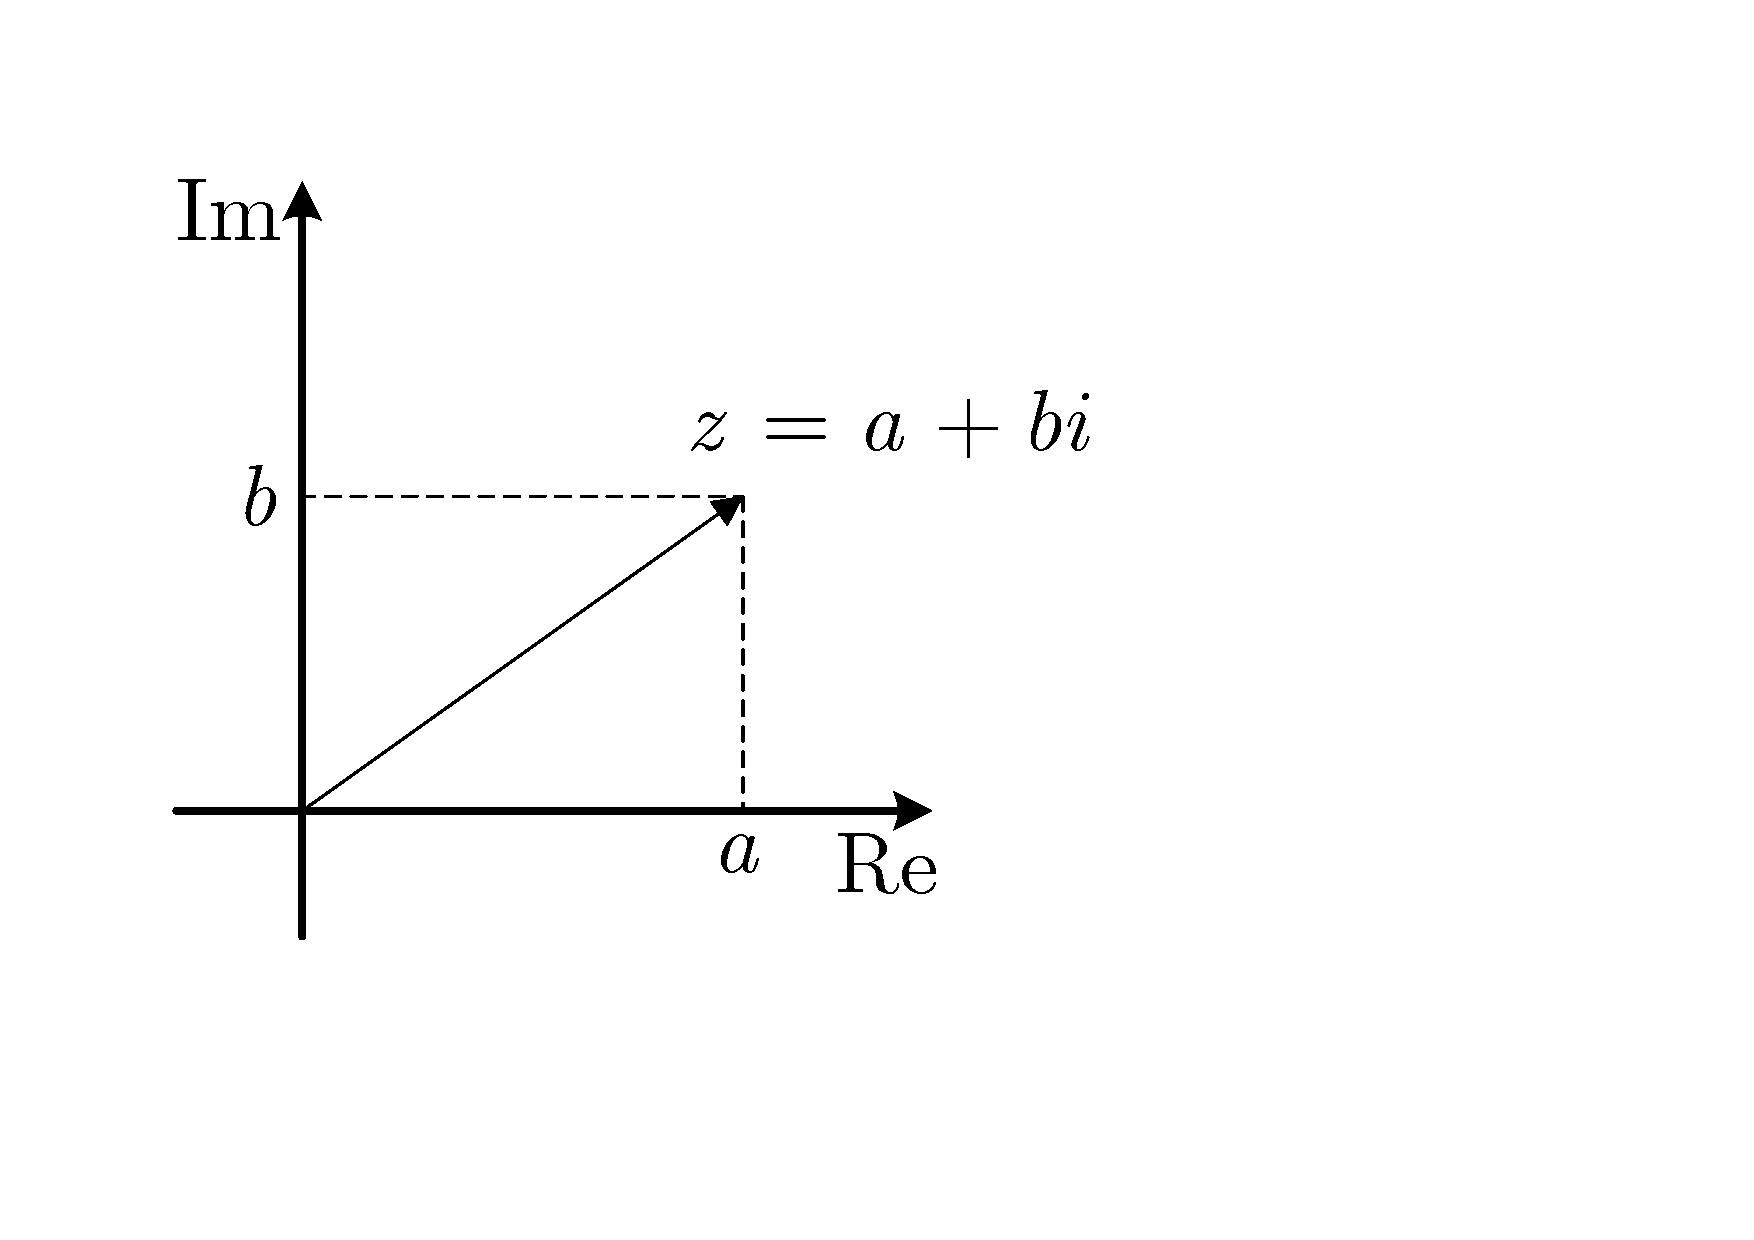
\includegraphics[width=0.3\textwidth]{complexPlane}
\caption{\label{complexPlane}complex plane}
\end{figure}

\begin{example}
$a+2+2bi = 3b+(a-1)i$일 때 $a$와 $b$를 구하시오.
\end{example}
\begin{proof}
$a+2 = 3b$, $2b = a-1$을 연립해 풀면 $a = 7$, $b = 3$.
\end{proof}

복소수의 덧셈, 뺄셈이 평면에서 벡터의 덧셈, 뺄셈과 같은 표현임을 알았다. 그렇다면 이번에는 복소수의 곱셈이 갖는 의미는 무엇인지 생각해 볼 필요가 있다. 우선 실수의 곱셈을 복소평면 상에서 생각해 보자 실수 1은 복소평면 상에서 $(1,0)$의 위치에 찍힌 점으로 표현된다. 여기에 $-1$을 곱하면 $(-1,0)$의 위치로 점이 이동하게 된다. 만약 $-1$을 곱하는 과정을 $i$를 두 번 곱하는 과정으로 생각한다면 $(1,0)$에 위치한 점이 반시계방향으로 $90^{\circ}$씩 두 번 회전한 것으로 생각할 수 있지 않을까? 이러한 생각이 맞는지 확인해 보자 1에 $i$를 한 번 곱하면 $1\cdot i = i$이고 이는 \myfig\ref{complexPlane}에서 $a = 0$, $b = 1$을 대입한 결과 이므로 $(0,1)$에 위치함을 알 수 있다. 앞서 생각했던 내용이 옳음을 직관적으로 알 수 있다.

이제 임의의 복소수끼리 곱했을 경우 어떠한 결과를 얻을 수 있는지 알아볼 차례이다. 그전에 $z = a+bi$의 다른 표현법을 알아보자. \myfig\ref{complexPlane}에서 원점으로부터 $z$까지 거리를 $r$이라 하고 실수축으로부터의 각을 $\theta$라 하면 $a = r \cos \theta$, $b = r \sin \theta$이므로 $z$를 다음과 같이 표현할 수 있다.
\begin{equation}
z = r(\cos\theta + i \sin\theta).
\end{equation}
이제 또 다른 복소수를 $z'$이라 하고 원점으로부터의 거리를 $r'$, $\Re$축으로부터의 각을 $\theta '$이라 하면 $z = r'(\cos\theta ' + i \sin\theta ')$ 으로 나타낼 수 있다. 이제 $z$와 $z'$을 곱해보면
\begin{align}
zz' &= rr' \left[ \cos\theta \cos\theta ' + i(\sin\theta \cos\theta ' + \cos\theta \sin\theta ') - \sin\theta \sin\theta ' \right]\nonumber
\\ &= rr' \left[ \cos (\theta+\theta ') + i \sin (\theta + \theta ') \right].
\end{align}
이 결과를 해석해 보면 두 복소수를 곱한 결과는 크기는 각각의 크기를 곱한 것과 같고 각은 각각의 각을 더한 것과 같음을 알 수 있다. 조금 전 1에 $i$를 곱하던 과정을 생각해 보면 $i$는 크기는 1이고 각은 $90^{\circ}$이므로 우리의 예상이 옳은 결과임을 알 수 있다. 복소수와 복소수 자신의 켤레복소수를 곱하면 어떻게 될까? $z = a+bi$와 $z$의 켤레복소수 $z^{\ast} = a-bi$를 곱하면 $zz^{\ast} = a^2 + b^2 = r^2$임을 알 수 있다. 즉 $\sqrt{zz^{\ast}} = r$이고 이를 $|z|$로 나타낸다. 즉,
\begin{equation}
|z| = \sqrt{zz^{\ast}}.
\end{equation}

복소수의 실수부와 허수부가 정해지면 그 복소수는 유일하게 하나로 결정된다. 마찬가지로 복소수의 크기와 각이 정해지면 그 복소수는 유일하게 하나로 결정된다. 따라서 복소수를 실수부와 허수부로 표현하는 대신 크기와 각으로 다음과 같이 표현하기도 한다.
\begin{equation}
z = |z|\angle \theta .
\end{equation}
$z = a+bi$와 같은 표현을 직각좌표형식이라 하고 $z = |z| \angle \theta$와 같은 표현을 극좌표형식이라 한다. 직관적으로 $z^{\ast} = |z|\angle-\theta$임을 알 수 있다.

\begin{example}
$z = \frac{1}{2} + \frac{\sqrt3}{2}i$를 극좌표형식으로 나타내시오.
\end{example}

\begin{proof}
$1 \angle 60^{\circ}$.
\end{proof}

\begin{example}
$z_1 = 3 \angle 22.5^{\circ}$, $z_2 = 5 \angle 75^{\circ}$일 때 $z_1 z_2$를 구하시오.
\end{example}

\begin{proof}
두 복소수를 곱한 결과는 크기끼리는 곱하고 각끼리는 더해주면 되므로 $z_1 z_2 = 3\cdot 5 \angle (25.5^{\circ}+75^{\circ}) = 15 \angle 100.5^{\circ}$.
\end{proof}

\begin{example}
$x^3 = -1$의 모든 근을 구하시오.
\end{example}

\begin{proof}
$x = r \angle \theta$라 하면 주어진 방정식은 $r^3 \angle 3\theta = 1 \angle \pi + 2\pi n$, $(n = 1,2,3,\cdots)$이 된다.(평면상의 점을 $360^{\circ}$회전시켜 보라 그 점의 위치가 바뀌는가...) $r$은 거리이므로 항상 양수이고 따라서 $r = 1$이다. $3\theta = \pi + 2\pi n$, $\theta = \frac{\pi}{3} + \frac{2\pi n}{3}$이므로 가능한 $\theta$의 값은 $\theta_1 = \frac{\pi}{3}$, $\theta_2 = \pi$, $\theta_3 = \frac{5\pi}{3}$이다.($n=3$인 경우부터는 결국 $\frac{\pi}{3}$, $\pi$, $\frac{5\pi}{3}$의 반복이므로...) 따라서 답은 $1 \angle \frac{\pi}{3}$, $1 \angle \pi$, $1 \angle \frac{5\pi}{3}$이다. 이를 직각좌표형식으로 표현하면 각각 $\frac{1}{2} + \frac{\sqrt3}{2}i$, $-1$, $\frac{1}{2} - \frac{\sqrt3}{2}i$이고 이는 주어진 방정식을 $(x+1)(x^2 - x + 1) = 0$로 인수분해 하고 근의 공식을 이용하여 구한 결과와 일치함을 알 수 있다.
\end{proof}


앞서 복소수의 덧셈에서 벡터와의 유사성을 보았다. 이러한 유사성을 또 하나 들어보려 한다. 두 벡터 $\vec{a}$, $\vec{b}$의 내적은 다음과 같이 정의한다.
\begin{equation}
\vec{a} \cdot \vec{b} = ab \cos\theta
\end{equation}
여기서 $|\vec{a}| = a$, $|\vec{b}| = b$이고 $\theta$는 두 벡터의 사이 각이다. 복소수에서도 이와 유사한 것을 나타낼 수 있다. $z_1 = |z_1| \angle \theta_1$, $z_2 = |z_2| \angle \theta_2$라 하면
\begin{align}
\mathbf{Re}\{z_1 z_2^{\ast}\} &= \mathbf{Re}\{ |z_1||z_2| \angle (\theta_1 - \theta_2)\}\nonumber \\
&= |z_1||z_2| \cos \theta, \quad (\theta = \theta_1 - \theta_2).
\end{align}
실수부 대신 허수부를 취하면 결과가 어떻게 될지 생각해 보고 이것은 어떤 것과 연관 지어 볼 수 있을지 생각해 보자.


%%%%%%%%%%%%%%%%%%%%%%%%%%%%%%%%%%%%%%%%%%%%%%%%%%%%%%
\section{복소수와 삼각함수의 관계}
이 내용에 관해서는 고등학교 수학의 범위를 벗어나지 않는 수준에서 어떻게 설명해야 할 지 모르겠다. 수학적으로 체계 있는 설명은 못하더라도 복소수와 삼각함수 간의 관계를 그럴듯하게라도 받아들이도록 설명하고자 한다.

$y = e^{ax}$를 생각해 보자 $\frac{dy}{dx} = a e^{ax} = ay$임은 이과생이라면 누구나 알 것이다. 그렇다면 이번에는 $z = \cos\theta + i\sin\theta$를 생각해 보자. $z$를 $\theta$에 관해 미분하면
\begin{equation}
\frac{dz}{d\theta} = -\sin\theta + i\cos\theta = i(\cos\theta + i\sin\theta) = iz.
\end{equation}
그렇다면 $y = e^{ax}$의 경우에 비추어 볼 때 $z = e^{i\theta}$가 아닐까? 여기서 이를 증명할 수는 없지만 이는 맞는 생각이다. 이로부터 복소수의 또 다른 표현을 얻었다.\footnote{오일러의 항등식이라 한다.}
\begin{equation} \label{eqEuler}
\cos\theta + i\sin\theta = e^{i\theta}.
\end{equation}
이제 우리는 복소수를 세 가지 형태로 나타낼 수 있다.
\begin{align}
\textrm{직각좌표 형식 : }&\; z = a+bi \nonumber \\
\textrm{극좌표 형식 : }&\; z = |z| \angle\theta \nonumber \\
\textrm{지수함수 형식 : }&\; z = re^{i\theta} \nonumber
\end{align}
이 세 가지 모두 복소수를 표현하는데 자주 사용된다.


\begin{figure}[!hbp]
\centering
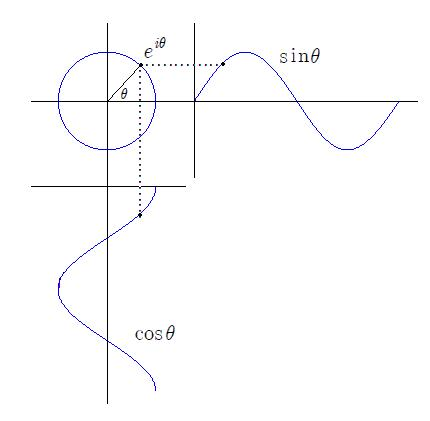
\includegraphics[width=0.5\textwidth]{sinevsexponential}
\caption{복소 지수함수와 삼각함수의 관계 도시}
\end{figure}

식 \eqref{eqEuler}에 $i$대신 $-i$를 대입하면 $\cos\theta - i\sin\theta = e^{-i\theta}$이다. 이제 둘을 더하거나 빼서 정리하면
\begin{align}
\cos\theta &= \frac{e^{i\theta} + e^{-i\theta}}{2}, \label{eqcos}\\
\sin\theta &= \frac{e^{i\theta} - e^{-i\theta}}{2i}. \label{eqsin}
\end{align}
이를 통해 지수함수와 삼각함수 사이의 관계를 얻었다. 식 \eqref{eqsin}의 우변을 $\theta$에 대해 미분해 식 \eqref{eqcos}의 우변이 됨을 확인해 보고 마찬가지로 식 \eqref{eqcos}\을 미분해 식 \eqref{eqsin}에 $-1$을 곱한 결과가 됨을 확인해 보자 이는 $\cos\theta$, $\sin\theta$에 대한 식 \eqref{eqcos}, 식 \eqref{eqsin}의 표현이 옳다는 간접적인 증거가 된다.

\begin{example}
다음 복소수들을 각각 극좌표 형식, 지수함수 형식으로 나타내시오.
\[ 2i,\; 1+i,\; 1-i,\; -1 \]
\end{example}

\begin{proof}
$2 \angle 90^{\circ}$, $2 e^{i \frac{\pi}{2}}$ // $\sqrt{2} \angle 45^{\circ}$, $\sqrt{2}e^{i\frac{\pi}{4}}$ // $\sqrt{2} \angle{-45^{\circ}}$, $\sqrt{2}e^{-i\frac{\pi}{4}}$ // $1\angle 180^{\circ}$, $e^{i\pi}$.\footnote{$e^{i\pi} = -1$을 정리하면 $e^{i\pi}+1 = 0$이다. 이 식에는 수학에서 중요한 다섯 가지의 상수 $e$, $i$, $\pi$, 1, 0가 모두 들어있다.}
\end{proof}
























%%%%%%%%%%%%%%%%%%%%%%%%%%%%%%%%%%%%%%%%%%%%%%%%
%\subsection{12}
%
%%%%%%%%%%%%%%%%%%%%%%%%%
%\subsubsection{12}
%
%%%%%%%%%%%%
%\paragraph{dd}


%\begin{figure}[!b]
%\centering
%\includegraphics[width=1\textwidth]{./img/MFCSerial}
%\caption{로봇}
%\label{Fig:LeaderFollowingBlockDiagram}
%\end{figure}


%\begin{figure}[!hbt]
%\centering \subfloat[ ]
%{\includegraphics[width=0.5\textwidth]{./img/stableFormation}}
%\centering \subfloat[ ]
%{\includegraphics[width=0.5\textwidth]{./img/stableFormationError}}
%\caption{ }
%\label{Fig:Stable}
%\end{figure}



%%%%%%%%%%%%%%%%%%%%%%%%%%%%%%%%%%%%%%%%%%%%%%%%%%%%%%%

%\begin{thebibliography}{99}
%\bibitem{REF:BishopIFAC2011}A. N. Bishop, ``Distributed Bearing-Only Quadrilateral Formation Control,'' \emph{Proceedings of the 18th World Congress The International Federation of Automatic Control}, pp. 4507--4512, 2011.
%
%\end{thebibliography}


\end{document}